% TODO: Proposal
\begin{figure*}
    \centering
    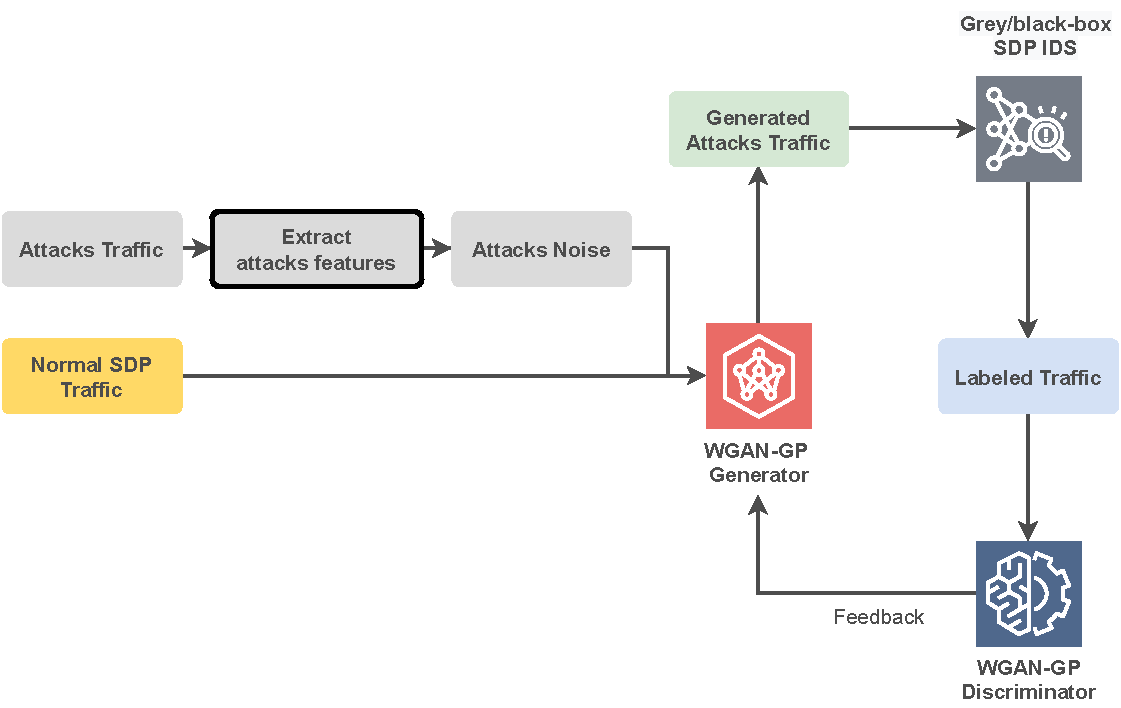
\includegraphics[width=.7\textwidth]{Figures/Harpe-WGAN-GP}
    \caption{\label{fig:harpe-architecture} \textit{Harpe} architecture.}
\end{figure*}

This research project proposes a new framework for generating malicious network traffic in
\textit{Software-Defined Perimeter (SDP)} based networks called \textit{Harpe}.
\textit{Harpe's} goal is to demonstrate that, although \textit{SDP}-based networks are much more secure than traditional
networks, they are not invulnerable and, further research is needed on how to improve them.
To demonstrate this, \textit{Harpe} generates malicious traffic that looks enough like normal traffic to fool the
\textit{Intrusion Detection System (IDS)} located in the \textit{SDP Controller}.
This \textit{IDS} is responsible for filtering traffic directed to the \textit{SDP Controller} (the only accessible
element of the architecture) and allowing only authorization and authentication requests, blocking possible attacks
such as denials of service, among others.

Generating malicious traffic that can fool an \textit{SDP's IDS} is not a simple task.
Creating network traffic that closely resembles normal traffic to evade detection can be difficult, as the limited
types of requests that are allowed make it challenging to create variations without being detected.
Furthermore, generating malicious traffic requires specific characteristics that are associated with successful
attacks.
These characteristics are not always easy to identify, as they can vary depending on the type of attack and the
\textit{IDS} being targeted.

\subsection{Harpe architecture}\label{subsec:traffic-generation}

The architecture of \textit{Harpe} is depicted in Figure~\ref{fig:harpe-architecture}.
In this architecture, The \textit{W-GAN} with Gradient Penalty is composed of two key elements: the
\textit{Traffic Generator} and the \textit{Discriminator}.

In order to generate malicious traffic data, the \textit{Harpe} framework requires access to two types of datasets: one
containing benign or normal \textit{SDP} traffic samples and another containing samples of known attack traffic.
A feature selection process is performed on the attack traffic samples to reserving the functional characteristics of
the traffic by taking into consideration the method in Usama’s study~\cite{usama2019generative}.
To generate adversarial traffic, the \textit{Traffic Generator} utilizes normal traffic as a base, and incorporates
noise derived from chosen features of known attack traffic.
The generated traffic is sent to the \textit{Grey/Black-box} \textit{IDS}, which only provides information on whether
or not the traffic is detected as an attack.
The generated traffic already labeled as benign or attack is passed to the \textit{Discriminator}.
The \textit{Discriminator} is a multi-layer neural network that is trained to distinguish between the normal traffic
and the generated adversarial traffic.
Also, the \textit{Discriminator} is trained to learn and imitate the \textit{IDS}’s decision process based on the
\textit{IDS}’s output.
Finally, the \textit{Discriminator} sends feedback to the \textit{Traffic Generator}, whose gradient is back-propagated
from the \textit{Discriminator} to improve the quality of the generated traffic.

\subsubsection{Feature selection}
In order to generate attacks on \textit{IDS} in network environments we have used the \textit{CIC-IDS2017},
\textit{CSE-CIC-IDS2018}, \textit{CIC-DDoS2019}, and \textit{UNSW-NB15} \textit{IDS} datasets.
These datasets contain benign and the most up-to-date common attacks, which resemble the true real-world data
(as \textit{PCAPs} files).
To generate the CSV files with which the framework works, we have used the
\textit{CICFlowmeter-V4.0}~\cite{lashkari2017cicflowmeter} tool from the Canadian Institute For Cybersecurity.
The \textit{CICFlowmeter-V4.0} is a tool that extracts features from \textit{PCAP} files and generates CSV files
as output.

After acquiring the necessary data, the next step is to identify the characteristics of the attacks that we want to
maintain during the generation of adversarial traffic.
The process of extracting features from traffic records for \textit{IDSs} is thoroughly discussed
by Lee et al~\cite{lee2000framework}.
The authors of this work have developed a four-layer feature extraction scheme that is based on the nature of the
attack found in network traffic flows.
These four steps of feature extraction are \textit{Intrinsic} features, \textit{Time-based} features,
\textit{Host-based} features, and \textit{Content-based} features.

The first step in the feature extraction process involves identifying \textit{intrinsic} features of the network
traffic flow.
These features are essential for determining the validity of the traffic and any alteration in these features will
render the traffic invalid.
The second step in the feature extraction process involves extracting \textit{time-based} features.
Any changes to the \textit{time-based} features of network traffic flow will invalidate the network traffic
characteristics.
Then, the \textit{host-based} traffic features were extracted and, in combination with \textit{intrinsic} and
\textit{time-based} features, are necessary for detecting \textit{slow-probe} attacks.
Any changes to these features will not only alter the \textit{host-based} information, but also invalidate the traffic
flow.
Finally, the content-based features are not required for denial of service attacks.
Any alteration in these features will not invalidate the attack.
In this framework, have used the content-based features to generate adversarial traffic.

\subsubsection{Data Generation}

\begin{equation}
    \label{eq:generatorloss}
    Gen_{Loss} = \mathbb{E}_{M \in normalData,N}Dis(M, N_{attacks})))
\end{equation}

The \textit{Traffic Generator} is a neural network with five linear layers, each with a \textit{ReLU} activation
function.
\textit{ReLU} is a rectified linear unit activation function that is used to add non-linearity to the
network ($ReLU(x) = \max(0, x)$).
The generator loss is calculated based on the \textit{Discriminator}’s output, which reflects the similarity between
the generated adversarial traffic and the normal traffic (see Equation~\ref{eq:generatorloss}).
The generator training performs updates to the generator’s weights based on the gradient information from the
similarity score.
The final goal is to minimize the generator loss.

\begin{equation}
    \label{eq:discriminatorloss}
    Dis_{Loss} = \mathbb{E}_{s \in P_{normal}}Dis(s) + \mathbb{E}_{s \in P_{attack}}Dis(s)
\end{equation}

The \textit{Discriminator} is a neural network with five linear layers, each with a \textit{LeakyReLU} activation
function ($LeakyReLU(x) = \max(0.01x, x)$).
The discriminator loss is calculated based on the results of the \textit{Grey/Black-box} \textit{IDS}’s output, which
labels the generated adversarial traffic as either benign or attack (see Equation~\ref{eq:discriminatorloss}).
The $P_{normal}$ and $P_{attack}$ are the normal and attack traffic samples predicted by the
\textit{IDS}, respectively.

\begin{table}[]
    \resizebox{0.8\columnwidth}{!}{%
        \begin{tabular}{lll}
            \hline
            \textbf{Operation} & \textbf{Units} & \textbf{Non-linearity} \\ \hline
            \multicolumn{3}{l}{\textbf{Traffic Generator (Gen)}} \\ \hline
            Linear             & $input\_dim$   & ReLU                   \\
            Linear             & $input\_dim//2$  & ReLU                   \\
            Linear             & $input\_dim//2$  & ReLU                   \\
            Linear             & $input\_dim//2$  & ReLU                   \\
            Linear             & $input\_dim//2$  & ReLU                   \\ \hline
            \multicolumn{3}{l}{\textbf{Discriminator (Dis)}} \\ \hline
            Linear             & $input\_dim$     & ReLU                   \\
            Linear             & $input\_dim\ast2$   & ReLU                   \\
            Linear             & $input\_dim\ast2$   & ReLU                   \\
            Linear             & $input\_dim\ast2$   & ReLU                   \\
            Linear             & $input\_dim//2$  & ReLU                   \\ \hline
        \end{tabular}
    }
    \caption{Architecture of the \textit{Traffic Generator} and \textit{Discriminator}.}
    \label{tab:gan_architecture}
\end{table}

\begin{table}[]
    \resizebox{0.7\columnwidth}{!}{%
        \begin{tabular}{ll}
            \multicolumn{2}{l}{\textbf{Hyperparameters}} \\ \hline
            Optimizer & RMSProp \\
            Learning Rate & 0.0001 \\
            Batch Size & 128 \\
            Iterations & 150 \\
            Weight Clipping & 0.01 \\
            Discriminator Iterations & 5 \\ \hline
        \end{tabular}
    }
    \caption{\textit{W-GAN} hyperparameters.}
    \label{tab:gan_hyperparameters}
\end{table}

The \textit{Generator} and \textit{Discriminator} architectures are described in Table~\ref{tab:gan_architecture},
and the \textit{W-GAN} hyperparameters are described in Table~\ref{tab:gan_hyperparameters}.

\subsubsection{Grey/Black-Box IDS}
The \textit{grey/black-box IDS} in our framework represents the \textit{ML-based IDS} used by the
\textit{SDP Controller} to filter incoming requests.
\textit{Harpe} only needs a binary response on the data it generates to label them as detected or undetected attacks.
To simulate this \textit{IDS}, we have used some of the most widely used and best performing classifiers from related
work.

\subsection{Integration with the SDP}\label{subsec:integration-with-the-sdp}

\begin{figure}
    \centering
    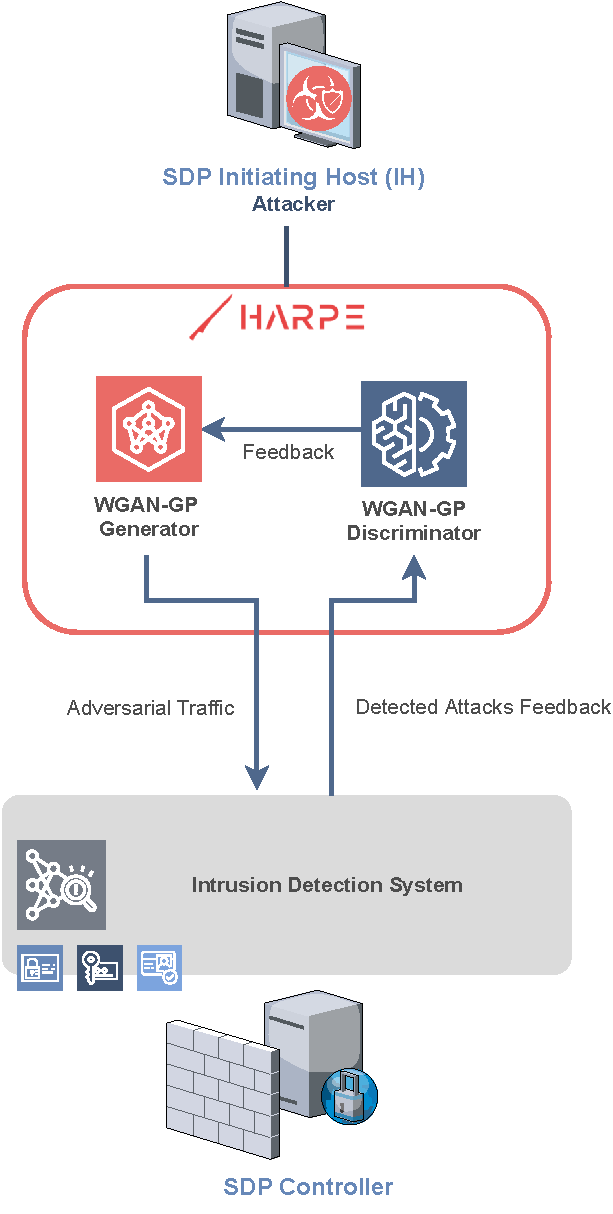
\includegraphics[width=.7\columnwidth]{Figures/Harpe-Integration}
    \caption{\label{fig:harpe-sdp-integration} \textit{Harpe} integration with the \textit{SDP}.}
\end{figure}

The \textit{Harpe} framework is integrated with the \textit{SDP} as shown in Figure~\ref{fig:harpe-sdp-integration}.
The attacker will correspond to the \textit{SDP IH} in the \textit{SDP} network architecture.
The \textit{SDP IH} will generate the adversarial traffic using the \textit{Traffic Generator} and send it to the
\textit{SDP Controller}.
Next, the \textit{IDS} will filter the incoming traffic and \textit{Harpe} will label the samples if they are
detected or undetected attacks.
The \textit{Discriminator} will be trained based on the \textit{IDS}’s output and send the updated weights to the
\textit{Traffic Generator}.
Once we have a trained \textit{Traffic Generator}, we can generate adversarial traffic that is similar to the
normal traffic and is undetected by the \textit{IDS}.

In a typical \textit{SDP} architecture, the \textit{SDP IH} needs to authenticate with the \textit{SDP Controller} to
gain access to the requested resources.
The only type of request in the \textit{SDP} network that can be attacked is the authentication step.
Authenticated requests between an \textit{SDP IH} and an \textit{SDP AH} typically have a short period of validity,
making it difficult for prolonged attacks such as denial of service \textit{(DoS)} to occur.
It should be noted that, in an \textit{SDP} network, there are two types of situations that make it difficult to carry
out attacks on the network.

\begin{itemize}
    \item The network is fully enclosed, where the components are fixed and cannot be altered.
    As a result, no external devices can initiate requests and to launch an attack, one must be part of the network.
    In this case, the locations and values of the \textit{SDP} IHs must be fixed and maintained throughout their
    lifetime in order to be connected to the network.

    \item The \textit{SDP} network allows for some flexibility in the \textit{SDP IH}, with the \textit{SDP Controller}
    being responsible for validation and verification.
    In this case, the \textit{SDP IH} can be moved to a different location, but the \textit{SDP Controller} must
    validate the new location.
    This case is the selected scenario for the \textit{Harpe} framework as it allows more requests types to train the
    \textit{Traffic Generator}.
\end{itemize}
